\section{Iterative Closest Point}

\subsection{ICP}
    \begin{frame}
        \frametitle{Buts}
        Pourquoi utiliser les nuages de points ?
        \begin{enumerate}
        	\item détection d'objets;
        	\item localisation;
        	\item odométrie (positionner le véhicule en mouvement);
        	\item cartographie;
        	\item etc.
		\end{enumerate}                   
    \end{frame}
    
    \begin{frame}
        \frametitle{Iterative Closest Point (ICP)}
        Algorithme permettant d'aligner deux nuages de points. Algorithme "point par point". 
            \begin{figure}              
                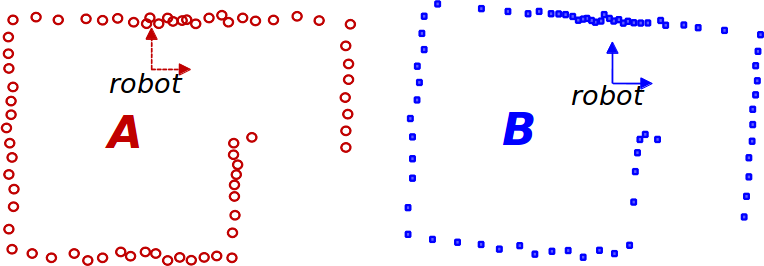
\includegraphics[width=\textwidth]{./media/init.png}
                \caption{Exemple de deux acquisitions d'une même pièce selon un point de vue différent}
            \end{figure}         
    \end{frame}
    
    \begin{frame}
        \frametitle{Iterative Closest Point (ICP)}
            \begin{figure}                 
                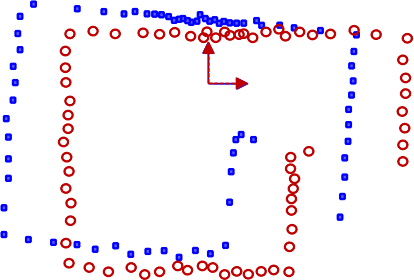
\includegraphics[width=0.6\textwidth]{./media/odom.png}
                \caption{Acquisitions sans alignement (centrées sur le robot)}
            \end{figure}
    \end{frame}
    
    \begin{frame}
        \frametitle{Iterative Closest Point (ICP)}
            \begin{figure}                 
                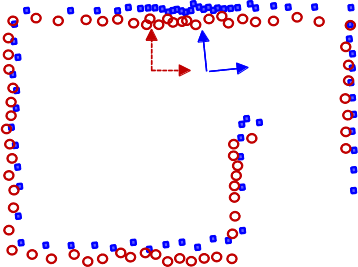
\includegraphics[width=0.6\textwidth]{./media/odom_adjusted.png}
                \caption{Acquisitions alignées en considérant l'odométrie du robot}
            \end{figure}
    \end{frame}
    
    \begin{frame}
        \frametitle{Iterative Closest Point (ICP)}
            \begin{figure}                 
                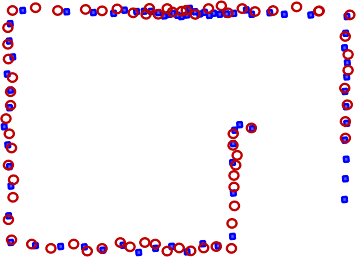
\includegraphics[width=0.6\textwidth]{./media/final.png}
                \caption{Alignement final ajusté grâce à ICP}
            \end{figure}
    \end{frame}
    
    \begin{frame}
    	\frametitle{Exemple en 3D}
    	\centering
    	\movie[showcontrols]{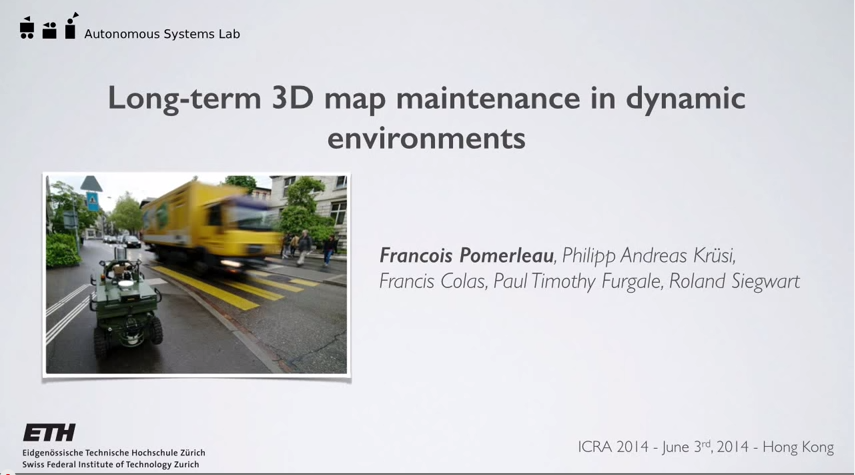
\includegraphics[width=\textwidth]{./media/vid.png}}{./media/icp_pomerleau.mp4}
    \end{frame}